\documentclass[12pt]{beamer}
\usepackage{../Estilos/BeamerMAF}
\input{../Preambulos/preambulo_Beamer_Dresden_seahorse}

\setbeamercolor{section in foot}{bg=ballblue, fg=black}
\setbeamercolor{subsection in foot}{bg=bronze, fg=black}
\setbeamercolor{date in foot}{bg=goldenrod, fg=white}

\makeatletter
\setbeamertemplate{footline}
{
\leavevmode%
\hbox{%
\begin{beamercolorbox}[wd=.333333\paperwidth,ht=2.25ex,dp=1ex,center]{section in foot}%
  \usebeamerfont{section in foot} \insertsection
\end{beamercolorbox}%
\begin{beamercolorbox}[wd=.333333\paperwidth,ht=2.25ex,dp=1ex,center]{subsection in foot}%
  \usebeamerfont{subsection in foot}  \insertsubsection
\end{beamercolorbox}%
\begin{beamercolorbox}[wd=.333333\paperwidth,ht=2.25ex,dp=1ex,right]{date in head/foot}%
  \usebeamerfont{date in head/foot} \insertshortdate{} \hspace*{1.5em}
  \insertframenumber{} / \inserttotalframenumber \hspace*{2ex} 
\end{beamercolorbox}}%
\vskip0pt%
}
\makeatother
\usefonttheme{serif}
\resetcounteronoverlays{saveenumi}

\date{7 de abril de 2022}

\title{\large{Expansión en eigenfunciones}}
\subtitle{Tema 3 - Bases completas y ortogonales}
\author{M. en C. Gustavo Contreras Mayén}


\begin{document}
\maketitle
\fontsize{14}{14}\selectfont
\spanishdecimal{.}

\section*{Contenido}
\frame[allowframebreaks]{\tableofcontents[currentsection, hideallsubsections]}

%ref. Herman (2015) 4.3 The eigenfunction expansion method

\section{Expansión en eigenfunciones}
\frame{\tableofcontents[currentsection, hideothersubsections]}
\subsection{Problema no  homogéneo}

\begin{frame}
\frametitle{El caso no homogéneo}
En esta sesión resolveremos el problema no homogéneo $\mathcal{L} \, y = f$ usando expansiones sobre la base de las eigenfunciones de Sturm-Liouville.
\\
\bigskip
\pause
Hemos visto que los problemas de eigenvalores de Sturm-Liouville tienen el conjunto necesario de eigenfunciones ortogonales.
\end{frame}
\begin{frame}
\frametitle{Técnica de expansión}
Aplicaremos el método de desarrollo de eigenfunciones para resolver un problema de valores en la frontera no homogéneo en particular.
\end{frame} 
\begin{frame}
\frametitle{La ED no homogénea}
Recordemos que iniciamos con una ecuación diferencial no homogénea:
\pause
\begin{align*}
\mathcal{L} \, y = f
\end{align*}
donde $y (x)$ debe satisfacer las condiciones de frontera homogéneas dadas.
\end{frame}
\begin{frame}
\frametitle{El método de expansión en eigenfunciones}
El método de expansión hace uso de las eigenfunciones que satisfacen el problema de eigenvalores:
\pause
\begin{align*}
\mathcal{L} \, \phi_{n} = - \lambda_{n} \, \sigma \, \phi_{n}
\end{align*}
sujeta a las condiciones de frontera dadas.
\end{frame}
\begin{frame}
\frametitle{Suposición inicial}
Entonces, suponemos que $y (x)$ se puede escribir como una expansión de las eigenfunciones:
\pause
\begin{align*}
y (x) = \nsum_{n=1}^{\infty} c_{n} \, \phi_{n} (x)
\end{align*}
y sustituimos la expansión en la ecuación no homogénea.
\end{frame}
\begin{frame}
\frametitle{Sustitución en la ED}
Esto nos da:
\pause
\begin{align*}
f (x) = \mathcal{L} \bigg( \nsum_{n=1}^{\infty} c_{n} \, \phi_{n} (x) \bigg) = - \nsum_{n=1}^{\infty} c_{n} \, \lambda_{n} \, \phi_{n} (x)
\end{align*}
\pause
Luego, los coeficientes de expansión $c_{n}$ se calculan haciendo uso de la ortogonalidad de las eigenfunciones.
\end{frame}
\begin{frame}
\frametitle{Calculando los coeficientes}
Es decir, multiplicamos la última ecuación por $\phi_{m} (x)$ y posteriormente integramos, obteniendo:
\pause
\begin{align*}
\scaleint{6ex}_{\bs a}^{b} &f (x) \, \phi_{m} (x) \dd{x} =  \\[0.5em]
&- \nsum_{n=1}^{\infty} c_{n} \, \lambda_{n} \, \scaleint{6ex}_{\bs a}^{b} \phi_{n} (x) \, \phi_{m} (x) \sigma (x) \dd{x}
\end{align*}
\end{frame}
\begin{frame}
\frametitle{La ortogonalidad nos favorece}
La ortogonalidad nos lleva a:
\pause
\begin{align*}
\scaleint{6ex}_{\bs a}^{b} f (x) \, \phi_{m} (x) \dd{x} = - c_{m} \, \lambda_{m} \, \scaleint{6ex}_{\bs a}^{b} \big[ \phi_{m} (x) \big]^{2} \, \sigma (x) \dd{x}
\end{align*}
\end{frame}
\begin{frame}
\frametitle{Los coeficientes buscados}
Resolviendo para $c_{m}$:
\pause
\begin{align*}
c_{m} = - \dfrac{\scaleint{6ex}_{\bs a}^{b} f (x) \, \phi_{m} (x) \dd{x}}{\lambda_{m} \, \scaleint{6ex}_{\bs a}^{b} \big[ \phi_{m} (x) \big]^{2} \, \sigma (x) \dd{x}}
\end{align*}
\end{frame}

\subsection{Ejemplo del método}

\begin{frame}
\frametitle{Enunciado del ejemplo}
Consideremos la solución del problema del valor en la frontera:
\pause
\begin{align}
(x \, \pderivada{y})^{\prime} + \dfrac{y}{x} = \dfrac{1}{x} \hspace{1.3cm} x \in [1, e] \label{eq:ecuacion_04_24} \\
y (1) = 0 = y (e) \label{eq:ecuacion_04_25}
\end{align}
Esta ecuación ya está en forma autoadjunta.
\end{frame}
\begin{frame}
\frametitle{Ventaja de ser una ecuación autoadjunta}
Entonces, sabemos que el problema de Sturm-Liouville de eigenvalores asociado tiene un conjunto ortogonal de eigenfunciones.
\\
\bigskip
\pause
Primero se tendrá que determinar éste conjunto.
\end{frame}
\begin{frame}
\frametitle{Problema a resolver}
Es decir, tenemos que resolver:
\pause
\begin{align}
(x \, \pderivada{\phi})^{\prime} + \dfrac{\phi}{x} = -\lambda \, \sigma \, \phi, \hspace{1.3cm} \phi (1) = 0 =\phi (e)
\label{eq:ecuacion_04_26}
\end{align}
\end{frame}
\begin{frame}
\frametitle{Manejando la expresión}
Organizando los términos y multiplicando por $x$, tenemos lo siguiente:
\pause
\begin{align*}
x^{2} \, \sderivada{\phi} + x \, \pderivada{\phi} + (1 + \lambda \, \sigma \, x) \, \phi = 0
\end{align*}
Esta es casi una ecuación del tipo de Cauchy-Euler.
\end{frame}
\begin{frame}
\frametitle{Eligiendo la función de peso}
Eligiendo la función de peso $\sigma (x) = 1 / x$, llegamos a:
\pause
\begin{align*}
x^{2} \, \sderivada{\phi} + x \, \pderivada{\phi} + (1 + \lambda ) \, \phi = 0
\end{align*}
Que fácilmente se puede resolver.
\end{frame}
\begin{frame}
\frametitle{Resolviendo la ED}
La ecuación característica es:
\pause
\begin{align*}
r^{2} + (1 + \lambda) = 0
\end{align*}
\pause
Se obtienen soluciones no triviales del problema de eigenvalores que satisfacen las condiciones de frontera cuando $\lambda > -1$.
\end{frame}
\begin{frame}
\frametitle{Soluciones a la ED}
Las soluciones son:
\pause
\begin{align*}
\phi_{n} (x) = A \, \sin (n \, \pi \, \ln x), \hspace{1.3cm} n = 1, 2, \ldots
\end{align*}
donde $\lambda_{n} = n^{2} \, \pi^{2} - 1$.
\end{frame}
\begin{frame}
\frametitle{Normalizando las eigenfunciones}
A menudo es útil normalizar las eigenfunciones.
\\
\bigskip
\pause
Esto significa que uno elige el valor de $A$ para que la norma de cada eigenfunción sea uno.
\end{frame}
\begin{frame}
\frametitle{Determinando la normalización}
Así, tenemos:
\pause
\begin{eqnarray}
\begin{aligned}[b]
1 &= \scaleint{6ex}_{\bs 1}^{e} \big[ \phi_{n} (x) \big]^{2} \, \sigma (x) \dd{x} = \\[0.5em] \pause
&= A^{2} \, \scaleint{6ex}_{\bs 1}^{e} \sin (n \, \pi \, \ln x) \, \dfrac{1}{x} \dd{x} = \\[0.5em] \pause
&= A^{2} \, \scaleint{6ex}_{\bs 0}^{1} \sin (n \, \pi \, y) \dd{y} = \pause \dfrac{1}{2} \, A^{2}
\end{aligned}
\label{eq:ecuacion_04_27}
\end{eqnarray}
Por lo que: $A = \sqrt{2}$.
\end{frame}
\begin{frame}
\frametitle{Gráfica de las eigenfunciones}
\begin{figure}[H]
    \centering
    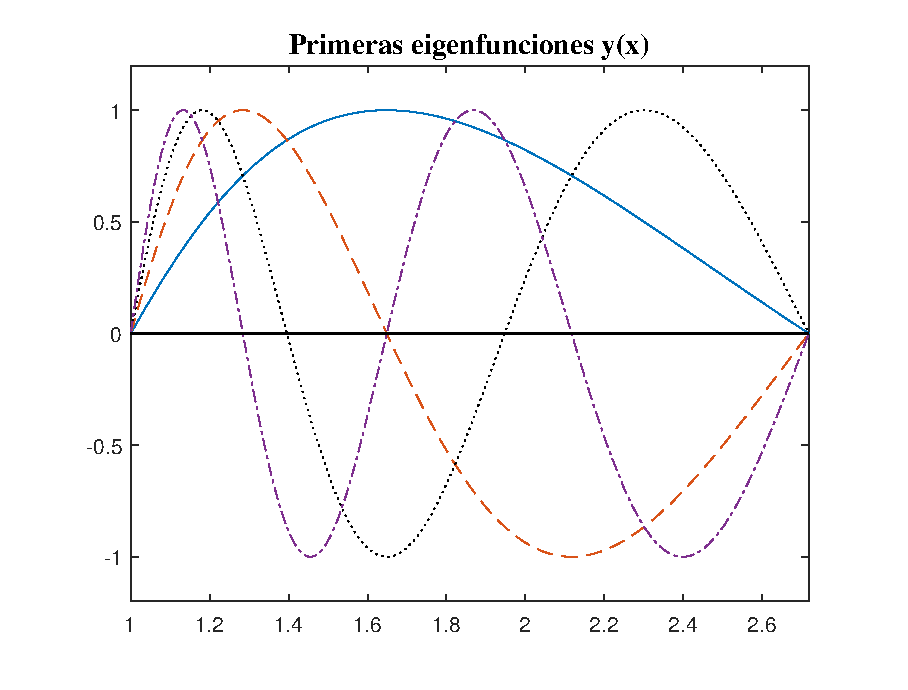
\includegraphics[scale=0.6]{Imagenes/Expansion_Eigenfunciones_01.eps}
    % \caption{Gráfica de las eigenfunciones del ejemplo.}
    % \label{fig:figura_04_02}
\end{figure}
\end{frame}
\begin{frame}
\frametitle{Avanzando en la solución}
Ahora nos enfocamos en resolver el problema no homogéneo $\mathcal{L} \, y = 1 / x$.
\\
\bigskip
\pause
Primero desarrollamos la solución desconocida en términos de las eigenfunciones:
\begin{align*}
y (x) = \nsum_{n=1}^{\infty} c_{n} \, \sqrt{2} \sin (n \, \pi \, \ln x)
\end{align*}
\end{frame}
\begin{frame}
\frametitle{Sustituyendo en la ED}
Sustituyendo esta solución en la ED, se tiene lo siguiente:
\pause
\begin{align*}
\dfrac{1}{x} = \mathcal{L} \, y = - \nsum_{n=1}^{\infty} c_{n} \, \lambda_{n} \, \sqrt{2} \, \sin (n \, \pi \, \ln x) \, \dfrac{1}{x}
\end{align*}
\end{frame}
\begin{frame}
\frametitle{Utilidad de la ortogonalidad}
Nuevamente usamos la ortogonalidad de las eigenfunciones, \pause para luego multiplicar ambos lados de la expresión por la eigenfunción:
\pause
\begin{align*}
\phi_{m} (x) = \sqrt{2} \, \sin (m \, \pi \, \ln x)
\end{align*}
\end{frame}
\begin{frame}
\frametitle{Integrando el resultado}
Posteriormente integramos, entonces tendremos que:
\pause
\begin{eqnarray*}
\begin{aligned}
\lambda_{m} \, c_{m} &= \scaleint{6ex}_{\bs 1}^{e} \sqrt{2} \, \sin (m \, \pi \, \ln x) \, \dfrac{1}{x} \dd{x} = \\[0.5em] \pause
&= \dfrac{\sqrt{2}}{m \, \pi} \, \big[ (-1)^{m} - 1 \big]
\end{aligned}
\end{eqnarray*}
\end{frame}
\begin{frame}
\frametitle{Obteniendo los coeficientes}
Resolviendo para los $c_{m}$:
\pause
\begin{align*}
c_{m} = \dfrac{\sqrt{2}}{m \, \pi} \, \dfrac{\big[ (-1)^{m} - 1 \big]}{m^{2} \, \pi^{2} - 1}
\end{align*}
\pause
Finalmente, sustituimos estos coeficientes en la expansión de $y (x)$. 
\end{frame}
\begin{frame}
\frametitle{Solución al problema}
La solución es entonces:
\pause
\begin{align*}
y (x) = \nsum_{n=1}^{\infty} \dfrac{2}{n \, \pi} \dfrac{\big[ (-1)^{n} - 1 \big]}{n^{2} \, \pi^{2} - 1} \sin (n \, \pi \, \ln x)
\end{align*}
\end{frame}
\begin{frame}
\frametitle{Gráfica de la  solución con $n=40$}
\begin{figure}[H]
    \centering
    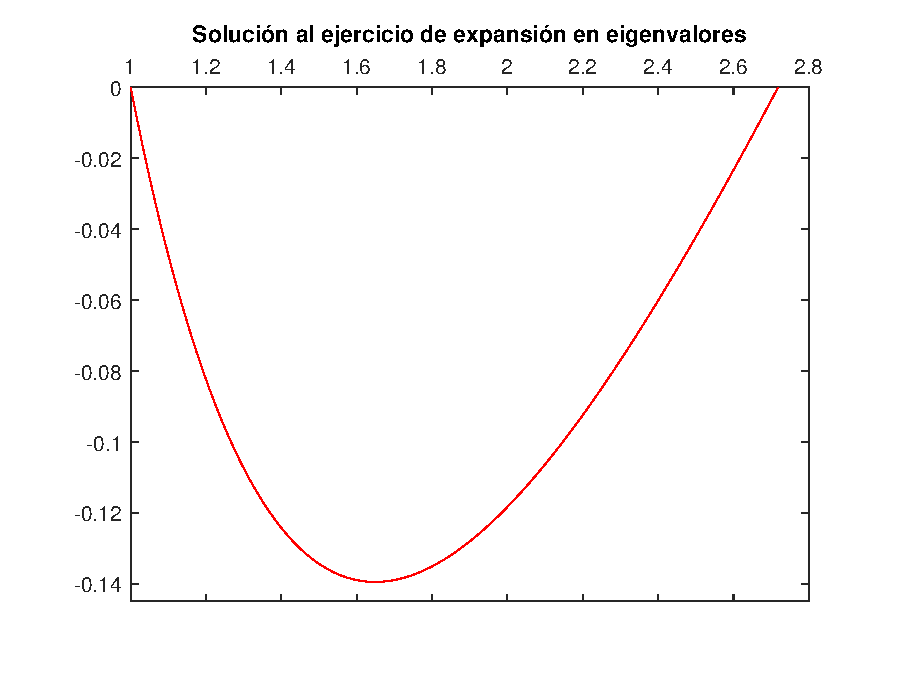
\includegraphics[scale=0.64]{Imagenes/Expansion_Eigenfunciones_02.eps}
    % \caption{Gráfica de la solución del ejemplo, se utilizó $n = 40$.}
    % \label{fig:figura_04_03}
\end{figure}
\end{frame}

% \section{Valores propios y operadores}
% \frame{\tableofcontents[currentsection, hideothersubsections]}
% \subsection{Valores y funciones propias}

% %Ref. Zettili Problem 2.18
% \begin{frame}
% \frametitle{Resolviendo un ejercicio }
% \setbeamercolor{item projected}{bg=blue!70!black,fg=yellow}
% \setbeamertemplate{enumerate items}[circle]
% \begin{enumerate}[<+->]
% \item Calcula los valores propios así como las funciones propias del operador $\hat{A} = - \dv*[2]{x}$.
% \\
% Limita la búsqueda de las funciones propias a aquellas funciones complejas que se anulan en todas partes excepto en la región $0 < x < a$.
% \item Normaliza la función propia y encuentra la probabilidad en la región $0 < x  < \dfrac{a}{2}$.
% \end{enumerate}
% \end{frame}
% \begin{frame}
% \frametitle{Resolviendo el inciso $\mathbf{1)}$}
% El problema de valores propios para $- \dv*[2]{x}$ consiste en resolver la siguiente ecuación diferencial:
% \pause
% \begin{align*}
% - \dv[2]{\psi}{x} = \alpha \, \psi (x)
% \end{align*}
% \pause
% y encontrar los valores propios $\alpha$ y las funciones propias $\psi (x)$.
% \end{frame}
% \begin{frame}
% \frametitle{Solución general a la EDO}
% Las solución más general para esta EDO es:
% \pause
% \begin{align*}
% \psi(x) = A \, \exp (i \, b \, x ) + B \, \exp (-i \, b \, x )
% \end{align*}
% con $\alpha = b^{2}$.
% \end{frame}
% \begin{frame}
% \frametitle{Usando las CDF}
% Ocupando las condiciones de frontera de $\psi(x)$ en $x = 0$ y en $x = a$, se tiene que:
% \pause
% \begin{eqnarray*}
% \begin{aligned}
% \psi (0) &= A + B = 0 \hspace{0.3cm} \Rightarrow \hspace{0.3cm} B = - A \\[0.5em] \pause
% \psi (a) &= A \, \exp (i b a) + B \, \exp(- i b a) = 0
% \end{aligned}
% \end{eqnarray*}
% \end{frame}
% \begin{frame}
% \frametitle{Usando los resultados}
% Al sustituir $B = - A$ en la segunda ecuación, nos lleva a:
% \pause
% \begin{eqnarray*}
% \begin{aligned}
% \psi (a) &= A \big[ \exp (i \, b \, a) - \exp(- i \, b \, a) \big] = 0 \\[0.5em] \pause
% \Rightarrow  \exp (i \, b \, a) &= \exp(- i \, b \, a) \big) \\[0.5em] \pause
% \Rightarrow  \exp (2 \, i \, b \, a) &= 1
% \end{aligned}
% \end{eqnarray*}
% \end{frame}
% \begin{frame}
% \frametitle{Calculando los valores propios}
% Por lo que:
% \pause
% \begin{eqnarray*}
% \begin{aligned}
% \sin ( 2 \, b \, a) &= 0 \\[0.5em] \pause
% \cos ( 2 \, b \, a) &= 1 \\[0.5em] \pause
% \Rightarrow b \, a &= n \, \pi
% \end{aligned}
% \end{eqnarray*}
% \end{frame}
% \begin{frame}
% \frametitle{Valores y funciones propias}
% Los valores propios son:
% \pause
% \begin{align*}
% \alpha_{n} = \dfrac{n^{2} \, \pi^{2}}{a^{2}}
% \end{align*}
% \pause
% Y las funciones propias son:
% \pause
% \begin{align*}
% \psi_{n}(x) = A \, \bigg[ \exp \bigg(\dfrac{i \, n \, \pi \, x}{a} \bigg) - \exp \bigg(- \dfrac{i \, n \, \pi \, x}{a} \bigg) \bigg]
% \end{align*}
% \end{frame}
% \begin{frame}
% \frametitle{Valores y funciones propias}
% Es decir que los valores propios y las funciones propias son:
% \pause
% \begin{align*}
% \setlength{\fboxsep}{3\fboxsep}\boxed{
% \alpha_{n} = \dfrac{n^{2} \, \pi^{2}}{a^{2}} \hspace{1cm} \psi_{n}(x) = C_{n} \, \sin \bigg(\dfrac{\, n \, \pi \, x}{a} \bigg) }
% \end{align*}
% \pause
% Por lo que el espectro de valores propios del operador $\hat{A} = - \dv*[2]{x}$ \textbf{es discreto}, ya que los valores propios y las funciones propias dependen de un número discreto $n$.
% \end{frame}
% \begin{frame}
% \frametitle{Resolviendo el inciso $\mathbf{2)}$}
% La normalización de las funciones propias $\psi_{n}(x)$ será tal que:
% \pause
% \begin{eqnarray*}
% \begin{aligned}
% 1 &= C_{n}^{2} \, \scaleint{6ex}_{\bs 0}^{a} \sin^{2} \bigg(\dfrac{n \, \pi \, x}{a} \bigg) \dd{x} = \\[0.5em] \pause
% &= \dfrac{C_{n}^{2}}{2} \scaleint{6ex}_{\bs 0}^{a} \bigg[ 1 - \cos \bigg(\dfrac{2 \, n \, \pi \, x}{a} \bigg) \bigg] \dd{x} = \\[0.5em] \pause
% &= \dfrac{C_{n}^{2}}{2} \, a
% \end{aligned}
% \end{eqnarray*}
% \end{frame}
% \begin{frame}
% \frametitle{Normalizando las funciones propias}
% Los que nos lleva a:
% \pause
% \begin{align*}
% C_{n} = \sqrt{\dfrac{2}{a}}
% \end{align*}
% \pause
% De aquí se obtienen las funciones propias normalizadas:
% \pause
% \begin{align*}
% \setlength{\fboxsep}{3\fboxsep}\boxed{
% \psi_{n}(x) = \sqrt{\dfrac{2}{a}} \, \sin \bigg(\dfrac{n \, \pi \, x}{a} \bigg) }
% \end{align*}
% \end{frame}
% \begin{frame}
% \frametitle{El valor de probabilidad}
% La probabilidad en la región $0 < x < \dfrac{a}{2}$ estará dada por:
% \pause
% \begin{eqnarray*}
% \begin{aligned}
% \dfrac{2}{a} \scaleint{6ex}_{\bs 0}^{\frac{a}{2}} &\sin^{2} \bigg(\dfrac{n \pi x}{a} \bigg) \dd{x} = \pause \dfrac{1}{a} \scaleint{6ex}_{\bs 0}^{\frac{a}{2}} \bigg[ 1 {-} \cos \bigg(\dfrac{2 n \pi x}{a} \bigg) \bigg] \dd{x} = \pause \dfrac{1}{2}
% \end{aligned}
% \end{eqnarray*}
% \pause
% Este se esperaba, ya que la probabilidad total es $1$:
% \begin{align*}
% \scaleint{6ex}_{0}^{a} \abs{\psi_{n} (x)}^{2} \dd{x} = 1
% \end{align*}
% \end{frame}

\section{Examen Intermedio}
\frame{\tableofcontents[currentsection, hideothersubsections]}
\subsection{Enunciados para el examen}

\begin{frame}
\frametitle{Los enunciados}
A continuación se enlistan los enunciados que formarán parte del Examen Intermedio, que cubre los temas 1, 2 y 3 del curso.
\end{frame}

\subsection{Tema 1}

\begin{frame}
\frametitle{Enunciados del Tema 1}
Para entregar:
\\
\bigskip
\pause
1, 2, 4, 6, 7, 8
\end{frame}

\subsection{Tema 2}

\begin{frame}
\frametitle{Enunciados del Tema 2}
Para entregar:
\\
\bigskip
\pause
1, 2, 3, 5, 6, 8
\end{frame}

\subsection{Tema 3}

\begin{frame}
\frametitle{Enunciados del Tema 3}
Hasta el contenido de normalización, faltaría 1 ejercicio que completa el Tema 3. 
\\
\bigskip
\pause
Se deben de entregar:
\\
\bigskip
\pause
1, 2, 3, 5, 8
\end{frame}

\subsection{Fecha de entrega}

\begin{frame}
\frametitle{Fecha de envío por Moodle}
La solución del examen con $17$ enunciados deberá de enviarse por Moodle el \textbf{martes 19 de abril a las 6 pm}
\end{frame}
\end{document}